\chapter{zad6}
\section{Optymalizacja regulatora PID}


W  celu optymalizacji użyta zostanie funkcja \emph{fmincon} z Matlaba. Znajduje ona lokalne minimum funkcji na podstawie jej gradientu. Aby użyc jej do optymalizacji regulatora PID zdefiniowano funkcję ewaluującą jakość regulacji, która zwraca wskaźnik jakości $E$, a jako argument bierze wektor nastaw $K$, $T_{\mathrm{i}}$ i $T_{\mathrm{d}}$ regulatora. Funkcja \emph{fmincon} będzie starała się ten wskaźnik zminimalizować, zaczynając od podanego przez nas wektora nastaw. Funkcja ewaluująca zwraca wskaźnik jakości regulacji $E$. Wywołanie funkcji \emph{fmincon} wyglądać może na przykład tak:

\begin{lstlisting}
%wywolanie funkcji ewaluujacej regulator PID
x01 = [1.975, 24, 3];   %punkt poczatkowy optymalizacji
fmincon(@pid_eval, x01)   %wywolanie funkcji
\end{lstlisting}

Po znalezieniu przez funkcję \emph{fmincon} minimum lokalnego, możemy wprowadzić te parametry do skryptu z poprzedniego zadania, i sprawwdzić czy rzeczywiście działają lepiej. Na rysunku 7.1 przedstawiono odnalezione przez funkcję \emph{fmincon} rozwiazanie. Widać jednak, że otrzymany regulator pracuje w stanie ciągłych oscylacji, i mimo że są one bardzo małe (na tyle małe, że nie sprawiają dużej różnicy dla wskaźnika jakości $E$), są one niepożądane na obiektach realnych. Regulator ten średnio więc się nadaje do zastosowania na obiekcie realnym. Sposobem na poprawę, mogłoby być wprowadzenie jakiegoś dodatkowego współczynnika kary za oscylacje wokół wartości zadanej, bądź duże wydłużenie czasu w której wartość zadana jest stała, żeby spróbować skłonić \emph{fmincon} do faworyzowania nieoscylujących regulatorów. Rys 7.2 przedstawia regulator otrzymany w wyniku optymalizacji funkcją \emph{fmincon} dla ośmiokrotnie wydłużonej symulacji. Zgodnie z oczekiwaniami, otrzymany regulator PID ma dużo mniejsze tendencje do oscylowania. Dla bardziej wydłużonej symulacji, powinno móc się uzyskać regulator dużo mniej podatny na oscylacje. Przez to jednak, wskaźnik jakości jest nieco gorszy.


\begin{figure}[tb] 
\centering 
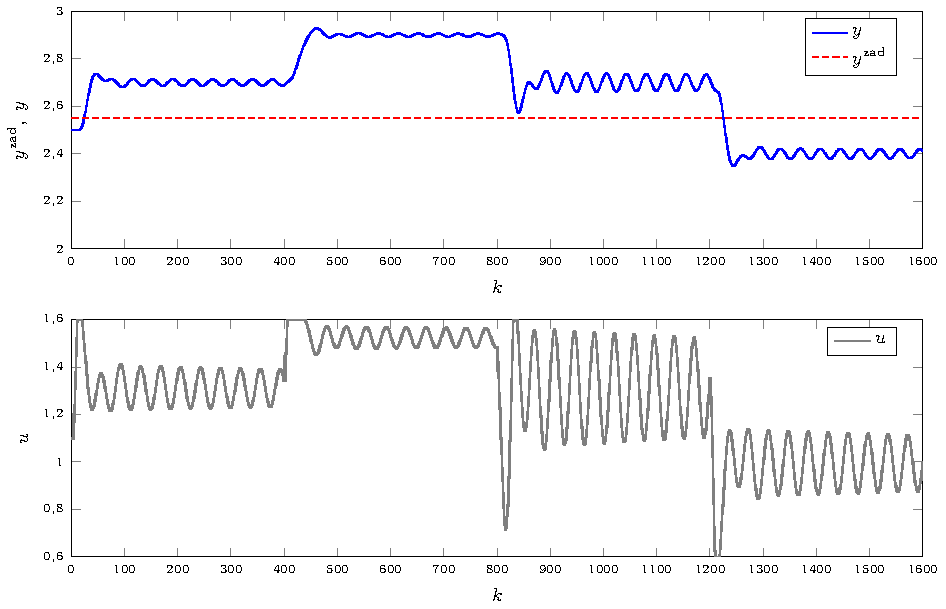
\includegraphics[scale=1]{rysunki/zapisz_pdf/PID_K=4.340_Ti=12.41_Td=8.10.pdf} 
\caption{Regulator PID $K=\num{4.34}$, $T_{\mathrm{i}}=12.41$, $T_{\mathrm{d}}=8.1$ otrzymany z punktu początkowego optymalizacji $K=\num{1.975}$, $T_{\mathrm{i}}=24$, $T_{\mathrm{d}}=3$} 
\label{r_pgfplots_PID_K=4.340_Ti=12.41_Td=8.10} 
\end{figure}

\begin{figure}[tb] 
\centering 
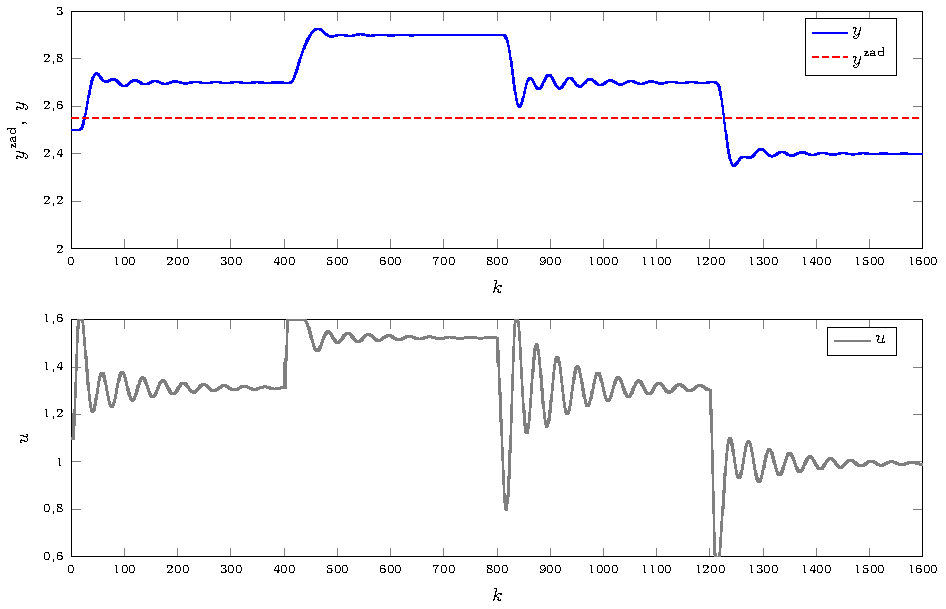
\includegraphics[scale=1]{rysunki/zapisz_pdf/PID_K=3.963_Ti=13.62_Td=7.87.pdf} 
\caption{Regulator PID $K=\num{3.963}$, $T_{\mathrm{i}}=13.62$, $T_{\mathrm{d}}=7.87$ otrzymany z punktu początkowego optymalizacji $K=\num{1.975}$, $T_{\mathrm{i}}=24$, $T_{\mathrm{d}}=3$} 
\label{r_pgfplots_PID_K=3.963_Ti=13.62_Td=7.87} 
\end{figure}




\begin{table}
	[b] \caption{Porównanie wielkości błędu $E$ dla różnych wartości parametru $T_{\mathrm{d}}$ i dla parametru $K=1.975$ oraz parametru $T_{\mathrm{i}}=24$}
	\label{t_T_i}
	\centering
	\sisetup{table-auto-round=true}
	\begin{small}
		\begin{tabular}{|c|c|c|c|}
			\hline
			$K$					&	$T_{\mathrm{i}}$	&	$T_{\mathrm{d}}$	&	$E$				\\
			$\num{4.3405}$		&	$\num{12.4148}$	&	$\num{8.097}$		&	$\num{5.0221}$	\\
			$\num{3.9628}$		&	$\num{13.6246}$	&	$\num{7.8695}$		&	$\num{5.1382}$	\\
			\hline
			\end{tabular}
	\end{small}
\end{table}

\section{Optymalizacja regulatora DMC}


W przypadku regulatora DMC niemożliwa jest optymalizacja funkcją \emph{fmincon}, ponieważ parametry regulatora DMC są zawsze dodatnimi liczbami całkowitymi. Z powodu użycia \emph{floor} w funkcji ewaluującej regulator DMC (analogiczna do funkcji ewaluującej regulator PID), funkcja \emph{fmincon} od razu zakończy optymalizację, twierdząc, że znalazła lokalne minimum. Jeżeli ma być odnaleziony najlepszy regulator DMC, należy użyć innej metody optymalizacji. Wybrana została funkcja \emph{ga} (,,Genetic Algorithm"), która jest częścią \emph{Global Optimization Toolbox} Matlaba. Wywołanie funkcji \emph{ga} może wyglądać tak:

\begin{lstlisting}
%wywolanie funkcji ewaluujacej regulator PID
x01 = [1.975, 24, 3];   %punkt poczatkowy optymalizacji
fmincon(@pid_eval, x01)   %wywolanie funkcji
%wywolanie funkcji ewaluujacej regulator DMC
A = [-1, 1];      
b = 0;          %ograniczenie liniowe -N+Nu<=0, czyli Nu<=N
Aeq = [];
beq = [];
lb = [1, 1];
ub = [200, 200];%ograniczenia wartosci N i Nu 1<=N<=200 i 1<=Nu<=200
nonlcon = [];
IntCon = [1, 2];    %pierwszy i drugi argument musza byc calkowite
ga(@dmc_eval,2,A,b,Aeq,beq,lb,ub,nonlcon,IntCon)
\end{lstlisting}

Tym spsobem otrzymaliśmy optymalne parametry regulatora DMC dla wybranej przez nas trajektorii wartości zadanej: $D=200$, $N=44$, $N_{\mathrm{u}}=5$. Regulator przedstawiony jest na Rys 7.3, a jego wskaźnik jakości $E=\num{4.6546}$. 

\begin{figure}[tb] 
\centering 
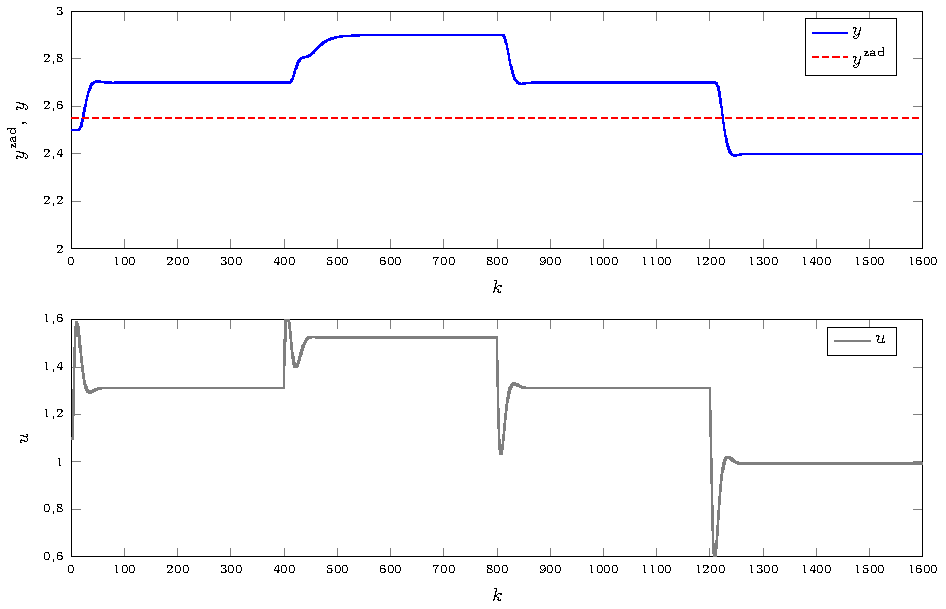
\includegraphics[scale=1]{rysunki/zapisz_pdf/DMC_D=200.000_N=44.00_Nu=5.00.pdf} 
\caption{Regulator DMC dla $D=200$, $N=44$, $N_{\mathrm{u}}=5$} 
\label{r_pgfplots_DMC_D=200.000_N=44.00_Nu=5.00} 
\end{figure}